\tikzset{every picture/.style={line width=0.75pt}} %set default line width to 0.75pt        

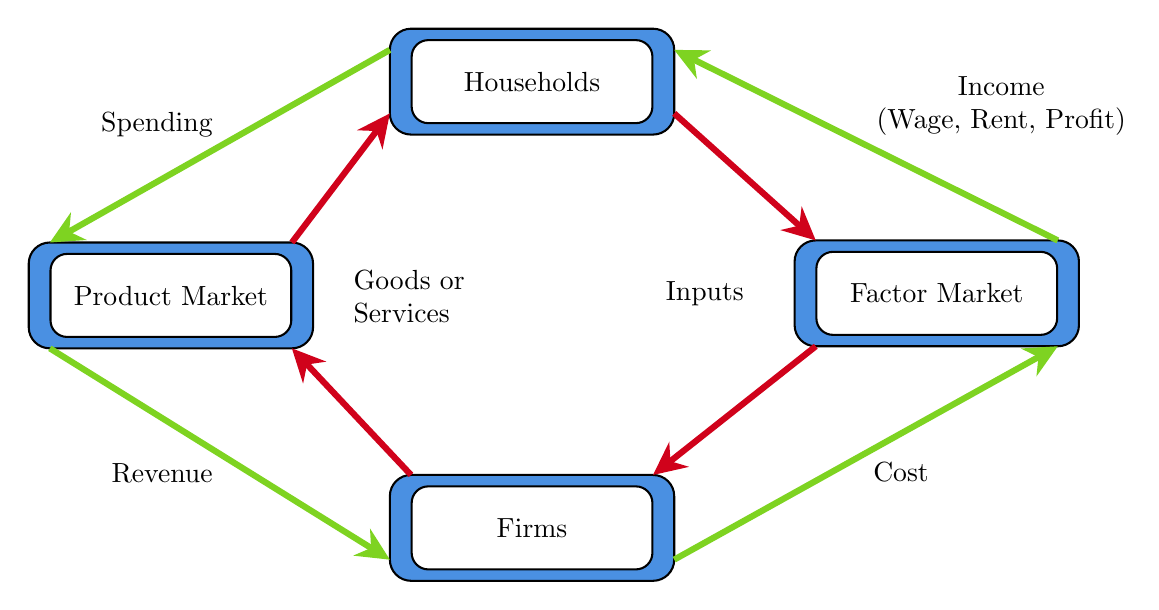
\begin{tikzpicture}[x=0.75pt,y=0.75pt,yscale=-1,xscale=1]
%uncomment if require: \path (0,300); %set diagram left start at 0, and has height of 300

%Rounded Rect [id:dp3465100630073805] 
\draw  [fill={rgb, 255:red, 74; green, 144; blue, 226 }  ,fill opacity=1 ] (263,22.2) .. controls (263,16.57) and (267.57,12) .. (273.2,12) -- (389.8,12) .. controls (395.43,12) and (400,16.57) .. (400,22.2) -- (400,52.8) .. controls (400,58.43) and (395.43,63) .. (389.8,63) -- (273.2,63) .. controls (267.57,63) and (263,58.43) .. (263,52.8) -- cycle ;
%Rounded Rect [id:dp7214464129129555] 
\draw  [fill={rgb, 255:red, 255; green, 255; blue, 255 }  ,fill opacity=1 ] (273.5,25.5) .. controls (273.5,21.08) and (277.08,17.5) .. (281.5,17.5) -- (381.5,17.5) .. controls (385.92,17.5) and (389.5,21.08) .. (389.5,25.5) -- (389.5,49.5) .. controls (389.5,53.92) and (385.92,57.5) .. (381.5,57.5) -- (281.5,57.5) .. controls (277.08,57.5) and (273.5,53.92) .. (273.5,49.5) -- cycle ;
%Rounded Rect [id:dp8133849265641938] 
\draw  [fill={rgb, 255:red, 74; green, 144; blue, 226 }  ,fill opacity=1 ] (458,124.2) .. controls (458,118.57) and (462.57,114) .. (468.2,114) -- (584.8,114) .. controls (590.43,114) and (595,118.57) .. (595,124.2) -- (595,154.8) .. controls (595,160.43) and (590.43,165) .. (584.8,165) -- (468.2,165) .. controls (462.57,165) and (458,160.43) .. (458,154.8) -- cycle ;
%Rounded Rect [id:dp30443809253463616] 
\draw  [fill={rgb, 255:red, 255; green, 255; blue, 255 }  ,fill opacity=1 ] (468.5,127.5) .. controls (468.5,123.08) and (472.08,119.5) .. (476.5,119.5) -- (576.5,119.5) .. controls (580.92,119.5) and (584.5,123.08) .. (584.5,127.5) -- (584.5,151.5) .. controls (584.5,155.92) and (580.92,159.5) .. (576.5,159.5) -- (476.5,159.5) .. controls (472.08,159.5) and (468.5,155.92) .. (468.5,151.5) -- cycle ;
%Rounded Rect [id:dp5907574749667166] 
\draw  [fill={rgb, 255:red, 74; green, 144; blue, 226 }  ,fill opacity=1 ] (89,125.2) .. controls (89,119.57) and (93.57,115) .. (99.2,115) -- (215.8,115) .. controls (221.43,115) and (226,119.57) .. (226,125.2) -- (226,155.8) .. controls (226,161.43) and (221.43,166) .. (215.8,166) -- (99.2,166) .. controls (93.57,166) and (89,161.43) .. (89,155.8) -- cycle ;
%Rounded Rect [id:dp5310892985635383] 
\draw  [fill={rgb, 255:red, 255; green, 255; blue, 255 }  ,fill opacity=1 ] (99.5,128.5) .. controls (99.5,124.08) and (103.08,120.5) .. (107.5,120.5) -- (207.5,120.5) .. controls (211.92,120.5) and (215.5,124.08) .. (215.5,128.5) -- (215.5,152.5) .. controls (215.5,156.92) and (211.92,160.5) .. (207.5,160.5) -- (107.5,160.5) .. controls (103.08,160.5) and (99.5,156.92) .. (99.5,152.5) -- cycle ;
%Rounded Rect [id:dp827002824816521] 
\draw  [fill={rgb, 255:red, 74; green, 144; blue, 226 }  ,fill opacity=1 ] (263,237.2) .. controls (263,231.57) and (267.57,227) .. (273.2,227) -- (389.8,227) .. controls (395.43,227) and (400,231.57) .. (400,237.2) -- (400,267.8) .. controls (400,273.43) and (395.43,278) .. (389.8,278) -- (273.2,278) .. controls (267.57,278) and (263,273.43) .. (263,267.8) -- cycle ;
%Rounded Rect [id:dp4820855032011546] 
\draw  [fill={rgb, 255:red, 255; green, 255; blue, 255 }  ,fill opacity=1 ] (273.5,240.5) .. controls (273.5,236.08) and (277.08,232.5) .. (281.5,232.5) -- (381.5,232.5) .. controls (385.92,232.5) and (389.5,236.08) .. (389.5,240.5) -- (389.5,264.5) .. controls (389.5,268.92) and (385.92,272.5) .. (381.5,272.5) -- (281.5,272.5) .. controls (277.08,272.5) and (273.5,268.92) .. (273.5,264.5) -- cycle ;
%Straight Lines [id:da22766006944212214] 
\draw [color={rgb, 255:red, 208; green, 2; blue, 27 }  ,draw opacity=1 ][fill={rgb, 255:red, 208; green, 2; blue, 27 }  ,fill opacity=1 ][line width=2.25]    (259.98,56.78) -- (215.8,115) ;
\draw [shift={(263,52.8)}, rotate = 127.19] [fill={rgb, 255:red, 208; green, 2; blue, 27 }  ,fill opacity=1 ][line width=0.08]  [draw opacity=0] (16.07,-7.72) -- (0,0) -- (16.07,7.72) -- (10.67,0) -- cycle    ;
%Straight Lines [id:da10983822042305391] 
\draw [color={rgb, 255:red, 126; green, 211; blue, 33 }  ,draw opacity=1 ][fill={rgb, 255:red, 126; green, 211; blue, 33 }  ,fill opacity=1 ][line width=2.25]    (263,22.2) -- (103.55,112.54) ;
\draw [shift={(99.2,115)}, rotate = 330.47] [fill={rgb, 255:red, 126; green, 211; blue, 33 }  ,fill opacity=1 ][line width=0.08]  [draw opacity=0] (16.07,-7.72) -- (0,0) -- (16.07,7.72) -- (10.67,0) -- cycle    ;
%Straight Lines [id:da13493886382595943] 
\draw [color={rgb, 255:red, 126; green, 211; blue, 33 }  ,draw opacity=1 ][fill={rgb, 255:red, 126; green, 211; blue, 33 }  ,fill opacity=1 ][line width=2.25]    (99.2,166) -- (258.75,265.16) ;
\draw [shift={(263,267.8)}, rotate = 211.86] [fill={rgb, 255:red, 126; green, 211; blue, 33 }  ,fill opacity=1 ][line width=0.08]  [draw opacity=0] (16.07,-7.72) -- (0,0) -- (16.07,7.72) -- (10.67,0) -- cycle    ;
%Straight Lines [id:da7517724119578088] 
\draw [color={rgb, 255:red, 208; green, 2; blue, 27 }  ,draw opacity=1 ][fill={rgb, 255:red, 208; green, 2; blue, 27 }  ,fill opacity=1 ][line width=2.25]    (219.23,169.64) -- (273.2,227) ;
\draw [shift={(215.8,166)}, rotate = 46.74] [fill={rgb, 255:red, 208; green, 2; blue, 27 }  ,fill opacity=1 ][line width=0.08]  [draw opacity=0] (16.07,-7.72) -- (0,0) -- (16.07,7.72) -- (10.67,0) -- cycle    ;
%Straight Lines [id:da36357253787164334] 
\draw [color={rgb, 255:red, 208; green, 2; blue, 27 }  ,draw opacity=1 ][fill={rgb, 255:red, 208; green, 2; blue, 27 }  ,fill opacity=1 ][line width=2.25]    (393.72,223.9) -- (468.2,165) ;
\draw [shift={(389.8,227)}, rotate = 321.66] [fill={rgb, 255:red, 208; green, 2; blue, 27 }  ,fill opacity=1 ][line width=0.08]  [draw opacity=0] (16.07,-7.72) -- (0,0) -- (16.07,7.72) -- (10.67,0) -- cycle    ;
%Straight Lines [id:da17368072688608072] 
\draw [color={rgb, 255:red, 208; green, 2; blue, 27 }  ,draw opacity=1 ][fill={rgb, 255:red, 208; green, 2; blue, 27 }  ,fill opacity=1 ][line width=2.25]    (400,52.8) -- (464.48,110.66) ;
\draw [shift={(468.2,114)}, rotate = 221.9] [fill={rgb, 255:red, 208; green, 2; blue, 27 }  ,fill opacity=1 ][line width=0.08]  [draw opacity=0] (16.07,-7.72) -- (0,0) -- (16.07,7.72) -- (10.67,0) -- cycle    ;
%Straight Lines [id:da6621718953660283] 
\draw [color={rgb, 255:red, 126; green, 211; blue, 33 }  ,draw opacity=1 ][fill={rgb, 255:red, 126; green, 211; blue, 33 }  ,fill opacity=1 ][line width=2.25]    (400,267.8) -- (580.43,167.43) ;
\draw [shift={(584.8,165)}, rotate = 510.91] [fill={rgb, 255:red, 126; green, 211; blue, 33 }  ,fill opacity=1 ][line width=0.08]  [draw opacity=0] (16.07,-7.72) -- (0,0) -- (16.07,7.72) -- (10.67,0) -- cycle    ;
%Straight Lines [id:da4548385579774181] 
\draw [color={rgb, 255:red, 126; green, 211; blue, 33 }  ,draw opacity=1 ][fill={rgb, 255:red, 126; green, 211; blue, 33 }  ,fill opacity=1 ][line width=2.25]    (404.48,24.42) -- (584.8,114) ;
\draw [shift={(400,22.2)}, rotate = 26.42] [fill={rgb, 255:red, 126; green, 211; blue, 33 }  ,fill opacity=1 ][line width=0.08]  [draw opacity=0] (16.07,-7.72) -- (0,0) -- (16.07,7.72) -- (10.67,0) -- cycle    ;
%Straight Lines [id:da014368688940361807] 
\draw [draw opacity=0]   (157.5,140.5) -- (242,141) ;
%Straight Lines [id:da27176174044752055] 
\draw [draw opacity=0]   (526.5,139.5) -- (437,139.5) ;

% Text Node
\draw (331.5,37.5) node   [align=left] {Households};
% Text Node
\draw (157.5,140.5) node   [align=left] {Product Market};
% Text Node
\draw (526.5,139.5) node   [align=left] {Factor Market};
% Text Node
\draw (331.5,252.5) node   [align=left] {Firms};
% Text Node
\draw (244,141) node [anchor=west] [inner sep=0.75pt]   [align=left] {Goods or\\Services};
% Text Node
\draw (435,139.5) node [anchor=east] [inner sep=0.75pt]   [align=left] {Inputs};
% Text Node
\draw (494.4,219.4) node [anchor=north west][inner sep=0.75pt]   [align=left] {Cost};
% Text Node
\draw (494.4,65.1) node [anchor=south west] [inner sep=0.75pt]   [align=left] {\begin{minipage}[lt]{92.5pt}\setlength\topsep{0pt}
\begin{center}
Income\\(Wage, Rent, Profit)
\end{center}

\end{minipage}};
% Text Node
\draw (179.1,219.9) node [anchor=north east] [inner sep=0.75pt]   [align=left] {Revenue};
% Text Node
\draw (179.1,65.6) node [anchor=south east] [inner sep=0.75pt]   [align=left] {Spending};


\end{tikzpicture}

